\chapter{Déploiement}
\noindent Nous avons décider de déployer le plugin sur le marketplace de Jetbrains.
Afin de permettre à tout le monde de pouvoir modifier le plugin, nous avons aussi décider de le mettre sur Github.


\section{Choix de la licence}
\noindent Nous avons choisi de mettre le plugin sous la licence MIT car elle est très permissive et permet à tout le monde de pouvoir modifier le plugin.
Une licence moins permissive aurait pu être la GNU GPLv3, mais elle impose de mettre le code source en open source et de mettre la licence dans le plugin.
\newdoubleline Voici un tableau comparatif des différentes licences que nous avons étudiées :

\begin{table}[H]
    \begin{tabular}{lccccc}
        \textbf{Permissions}    & \multicolumn{1}{l}{MIT} & \multicolumn{1}{l}{GNU GPLv3} & \multicolumn{1}{l}{GNU LGPLv3} & \multicolumn{1}{l}{Mozilla Public 2.0} & \multicolumn{1}{l}{Apache 2.0} \\
        Utilisation commerciale & x                               & x                             & x                              & x                                              & x                                      \\
        Utilisation privée      & x                               & x                             & x                              & x                                              & x                                      \\
        Distribution            & x                               & x                             & x                              & x                                              & x                                      \\
        Modification            & x                               & x                             & x                              & x                                              & x                                      \\
        \textbf{Conditions}     &                                 &                               &                                &                                                &                                        \\
        Indiquer la source      &                                 & x                             & x                              & x                                              &                                        \\
        Même licence            &                                 & x                             & x                              & x                                              &                                        \\
        \begin{tabular}[c]{@{}l@{}}
            Indiquer la licence \\ et le copyright
        \end{tabular} & x & x & x & x & x
    \end{tabular}
\end{table}

\section{Déploiement sur le marketplace}
\noindent Pour déployer le plugin sur le marketplace, il faut créer un compte sur le site de Jetbrains.
Une fois le compte créé, il suffit de se rendre sur la page de déploiement du plugin, de choisir le plugin à déployer et de remplir les informations demandées.
\newdoubleline Voici un exemple de ce que l'on peut voir sur la page de déploiement du plugin :

\begin{figure}[H]
    \centering
    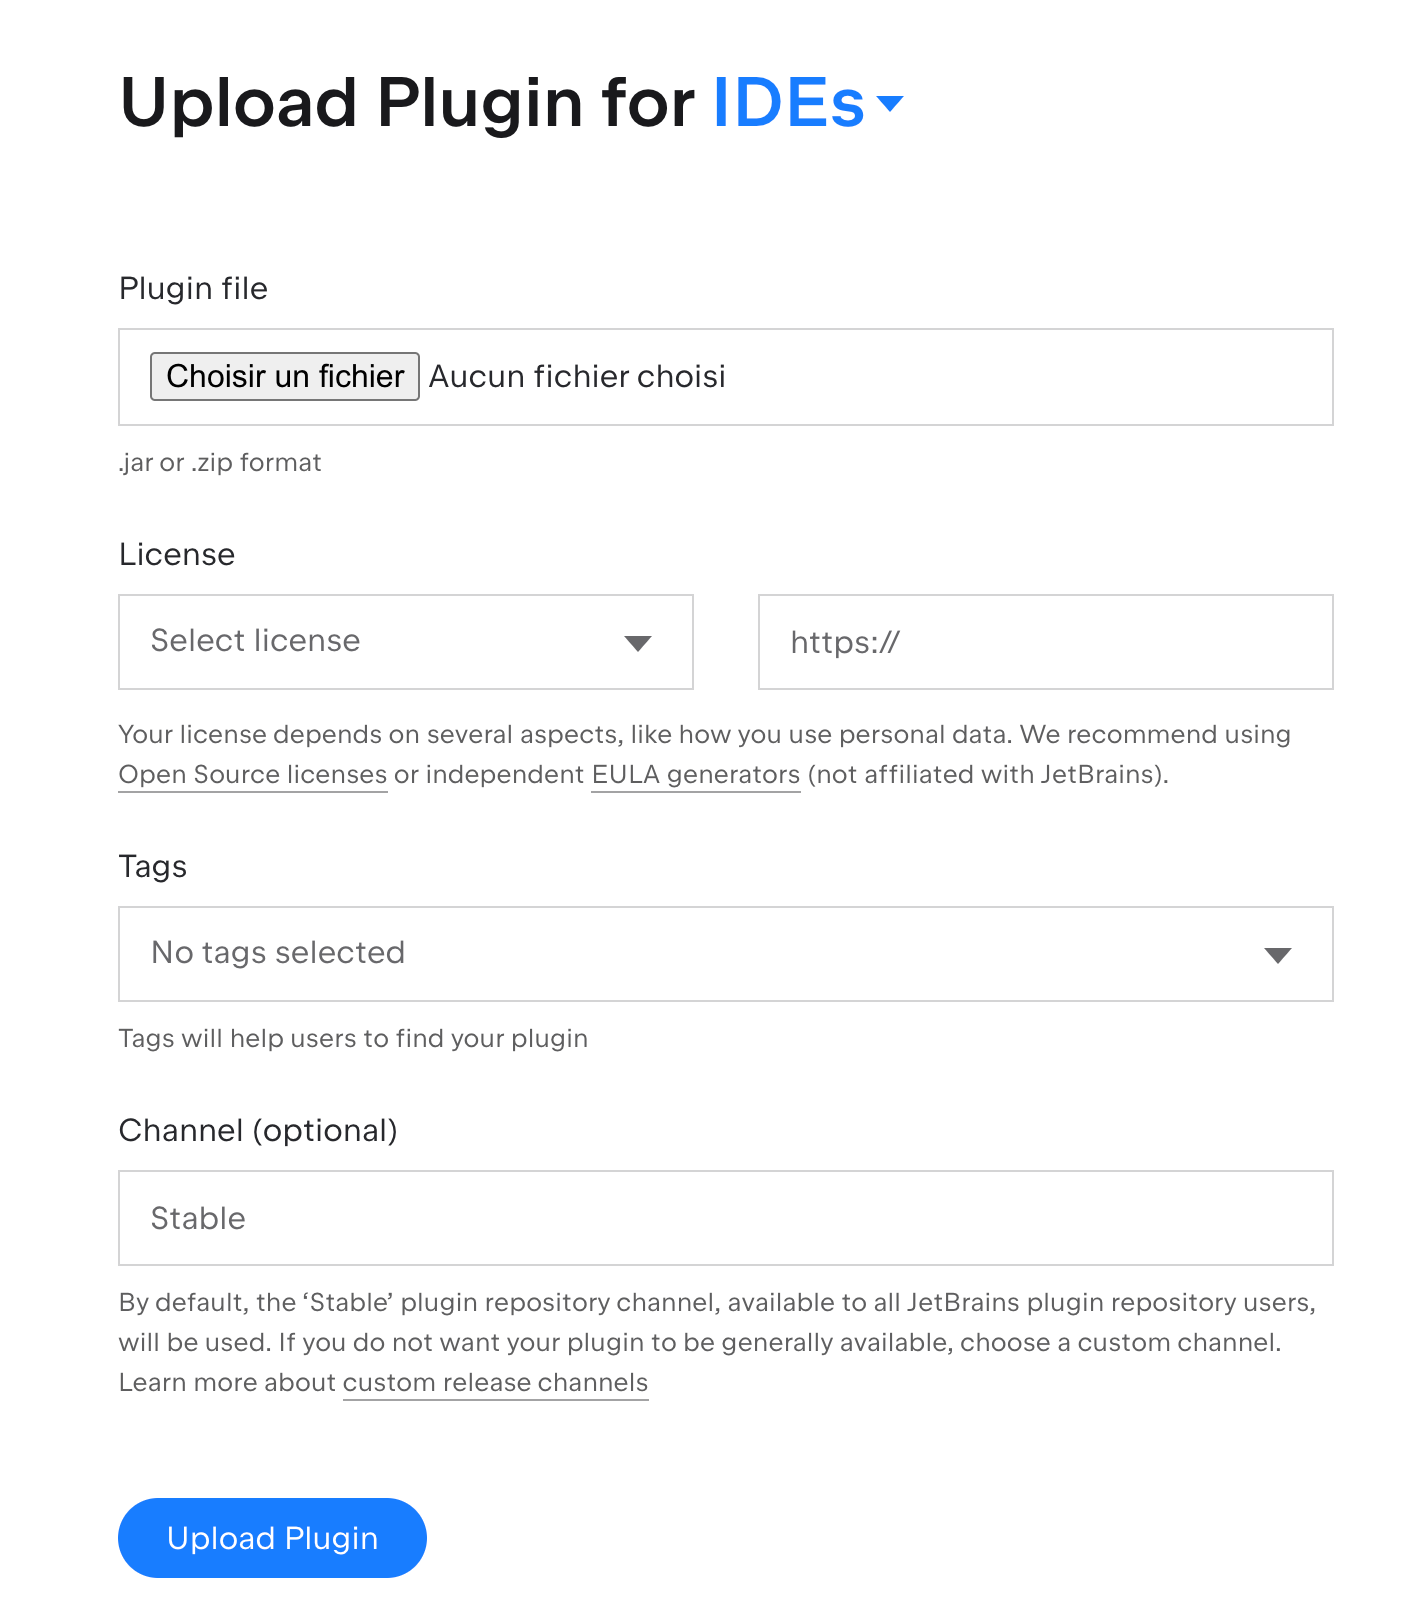
\includegraphics[width=0.5\textwidth]{images/first_deploy.png}
    \caption{Premier déploiement du plugin}
    \label{fig:first_deploy}
\end{figure}

\noindent Lors des déploiements suivants, il suffit de cliquer sur le bouton « Update » et de choisir le fichier .zip du plugin.
\newdoubleline La page du plugin sur le marketplace est la suivante : \url{https://plugins.jetbrains.com/plugin/20982-prologcode}
\newdoubleline Au moment où ce rapport est écrit, le plugin n'a pas encore été approuvé en raison du nom (IntelliProlog). Le nom ne devant pas faire référence à JetBrains ou l'un de ses produits, le plugin va être renommé et le plugin devrait être approuvé.

\section{Déploiement sur Github}
\noindent Une organisation Github a été créée pour le projet.
Le projet a été publié à l'adresse suivante: \url{https://github.com/IntelliProlog/IntelliProlog}


